%%=============================================================================
%% Conclusie
%%=============================================================================

\chapter{Conclusie}
\label{ch:conclusie}
In dit hoofdstuk worden de verschillende \glspl{tool} die in het vorige hoodstuk getest werden, vergeleken op vlak van:
\begin{itemize}
\item populariteit
\item syntax
\item mogelijkheden voor cross-browser testen en integratie met cloud services
\item mogelijkheden voor integratie in een \gls{CI} systeem
\item mogelijkheden voor het parallel uitvoeren van testen
\item performantie
\end{itemize}
Hierna wordt de conclusie geformuleerd en wordt toegelicht welke \gls{tool} verkozen werd en in het volgende hoofdstuk als toepassing voor Dropsolid gebruikt wordt.

\clearpage
\section{Vergelijking}
\subsection{Populariteit}
\begin{figure}[h]
\caption{Aantal wekelijkse downloads met Npm op een tijdspanne van 1 jaar, grafiek van \textcite{npmtrends}}
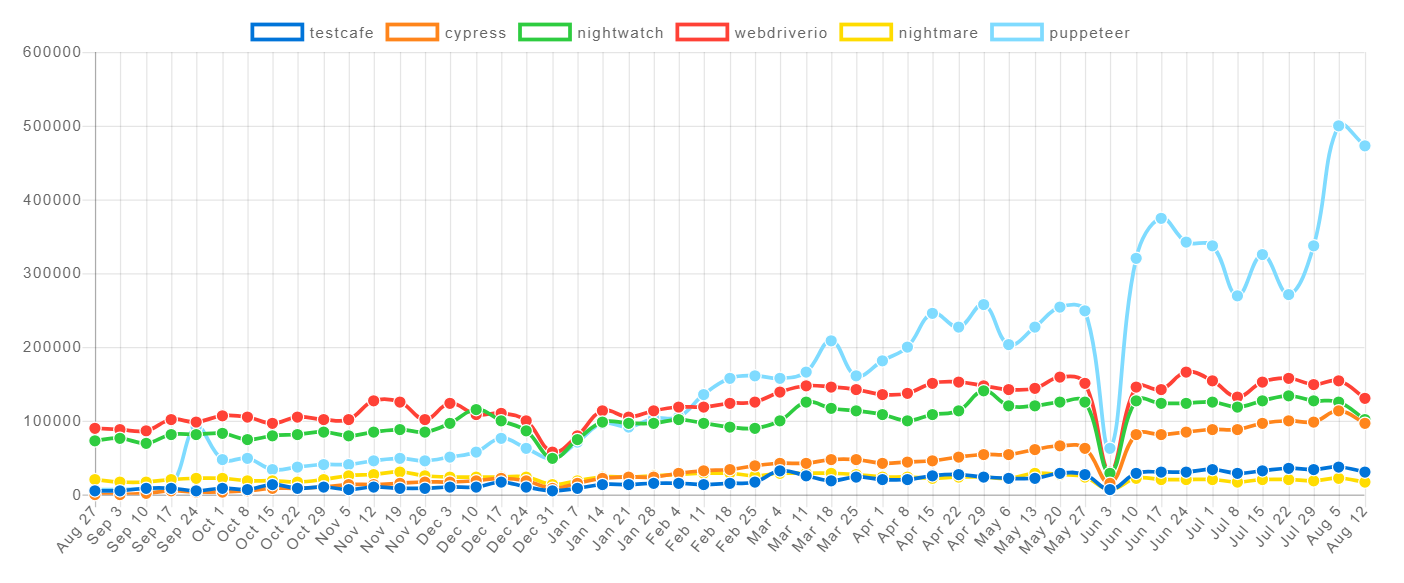
\includegraphics[width=1\textwidth]{img/npm_trends.PNG}
\end{figure}
Puppeteer heeft de sterkste groei meegemaakt sinds de \gls{tool} in januari van 2018 publiek werd gemaakt, met een piek van bijna 500000 wekelijkse downloads op 5 augustus. De drie populairste \glspl{tool} na Puppeteer met tussen de 100000 en 150000 wekelijkse downloads zijn WebdriverIO, Nightwatch en Cypress waarvan die laatste een langzame maar stabiele groei kende gedurende het afgelopen jaar. Nightmare en TestCafé zijn het minst populair met onder de 50000 wekelijkse downloads.

\subsection{Syntax}
TestCafé en Nightwatch zijn op vlak van syntax zeer gelijkaardig en zijn duidelijk te verstaan. Dit komt door de mogelijkheid om commando's te ketenen en om \glspl{assertie} zonder de ketting te breken uit te voeren. Kort daarop volgt WebdriverIO die ook zeer gelijkaardig is maar waarbij de ketting moet gebroken worden om \glspl{assertie} te maken.

Cypress code is ook goed verstaanbaar maar is net iets minder dan de voorgaande \glspl{tool} omdat opdrachten niet kunnen geketend worden.

Nightmare en Puppeteer zijn het minst goed leesbaar. Nightmare omdat de \glspl{assertie} niet met een simpel commando kunnen gemaakt worden en Puppeteer omdat de opdrachten niet kunnen geketend worden en er dus overal gebruik moet gemaakt worden van await zodat de commando's niet parallel uitgevoerd worden.

\subsection{Cross-browser en cloud service mogelijkheden}
\begin{tabular}{ | l | p{12cm} | }
\hline
 TestCafé & TestCafé ondersteunt het testen op Google Chrome, Internet Explorer, Microsoft Edge, Mozilla Firefox, Safari en Android. Ook kan TestCafé gebruik maken van alle bekende cloud services voor cross-browser testen zoals SauceLabs, Browserstack en TestingBot.\\
\hline
 Cypress & Cross-browser testen is momenteel niet mogelijk met Cypress, enkel Chrome varianten worden ondersteund. Er zijn wel plannen om in de toekomst meerdere browsers te ondersteunen, \textcite{Mann2017}. Momenteel is er ook nog geen integratie met cloud services mogelijk.\\
\hline
 Nightwatch & Integratie met alle bekende cloud services (BrowserStack, SauceLabs, TestingBot en CrossBrowserTesting) en alle bekende browsers (Google Chrome, Mozilla Firefox, Microsoft Edge en Internet explorer) is mogelijk.\\
\hline
 WebdriverIO & Integratie met alle bekende cloud services en alle bekende browsers is mogelijk.\\
\hline
 Nightmare & Nightmare kan enkel gebruik maken van de Electron applicatie en er zijn geen integratie mogelijkheden met cloud services.\\
\hline
 Puppeteer & Puppeteer ondersteund enkel Chrome en Chromium. Wel zijn er integratie mogelijkheden met de bekende cloud services.\\
\hline
\end{tabular}

\subsection{Integratie mogelijkheden met CI systemen}
\begin{tabular}{ | l | p{12cm} | }
\hline
 TestCafé & Voorziet documentatie voor integratie in AppVeyor, CircleCI, Jenkins, TeamCity en Travis.\\
\hline
 Cypress & Voorziet documentatie voor integratie in Jenkins, Travis, CircleCI en CodeShip.\\
\hline
 Nightwatch & Voorziet geen documentatie voor integratie in \gls{CI} systemen, wel zijn online voorbeelden te vinden over de integratie in de bekende \gls{CI} systemen zoals Jenkins en Travis. \\
\hline
 WebdriverIO & Voorziet documentatie voor integratie in Jenkins.\\
\hline
 Nightmare & Voorziet geen documentatie voor integratie in \gls{CI} systemen, wel zijn online voorbeelden te vinden over de integratie in de bekende \gls{CI} systemen.\\
\hline
 Puppeteer & Voorziet geen documentatie voor integratie in \gls{CI} systemen, wel zijn online voorbeelden te vinden over de integratie in de bekende \gls{CI} systemen.\\
\hline
\end{tabular}
\subsection{Parallel uitvoeren van testen}
\begin{tabular}{ | l | p{12cm} | }
\hline
 TestCafé & Het parallel uitvoeren van testen met TestCafé is standaard mogelijk.\\
\hline
 Cypress & Het parallel uitvoeren van testen met Cypress is momenteel nog niet mogelijk, hier wordt wel aan gewerkt.\\
\hline
 Nightwatch & Het parallel uitvoeren van testen met Nightwatch is standaard mogelijk. \\
\hline
 WebdriverIO & Het parallel uitvoeren van testen met Nightwatch is standaard mogelijk.\\
\hline
 Nightmare & Het parallel uitvoeren van testen met Nightmare is niet mogelijk.\\
\hline
 Puppeteer & Het parallel uitvoeren van testen met Nightmare is standaard niet mogelijk. Er zijn wel \glspl{library} door de community gemaakt om deze functionaliteit te voorzien zoals bijvoorbeeld Puppeteer Cluster.\\
\hline
\end{tabular}

\subsection{Performantie}

Deze tijden moeten niet gezien worden als een benchmark om de \glspl{tool} te vergelijken maar eerder als een proof of concept.

\begin{tabular}{ | l | p{12cm} | }
\hline
 TestCafé & Gemiddeld 12,3 seconden voor het uitvoeren van de test.\\
\hline
 Cypress & Gemiddeld 6,64 seconden voor het uitvoeren van de test.\\
\hline
 Nightwatch & Gemiddeld 5,5 seconden voor het uitvoeren van de test. \\
\hline
 WebdriverIO & Gemiddeld 6,64 seconden voor het uitvoeren van de test.\\
\hline
 Nightmare & Gemiddeld 8,69 seconden voor het uitvoeren van de test.\\
\hline
 Puppeteer & Gemiddeld 5,13 seconden voor het uitvoeren van de test.\\
\hline
\end{tabular}

\clearpage
\section{Conclusie}
De \gls{tool} die uit dit onderzoek naar voor komt als beste voor een \gls{KMO} gespecialiseerd in Drupal is Nightwatch. Nightwatch haalde het tweede beste resultaat op de performantietest en kan testen parallel uitvoeren. Er zijn voldoende mogelijkheden voor integratie met cloud services en ook cross-browser testen is geen probleem. Momenteel is er zelfs een cloud service specifiek voor Nightwatch in ontwikkeling. Ook de integratie in \gls{CI} systemen is geen probleem.

Nightwatch voorziet standaard de mogelijkheid om \gls{BDD} en unit testen te schrijven en heeft al een \gls{assertie} \gls{library} ingebouwd. Er is ook de mogelijkheid om screenshots te nemen met een eenvoudig commando.

De doorslaggevende factor was echter het feit dat de Drupal community naar deze \gls{tool} toegroeit voor het maken van hun functionele testen. Zo is Nightwatch opgenomen in de core van de voorlopige versie van Drupal 8.6. Er zijn al enkele commando's met Nightwatch ontwikkeld voor bijvoorbeeld het inloggen of uitloggen op een Drupal site te automatiseren.

%% TODO: Trek een duidelijke conclusie, in de vorm van een antwoord op de
%% onderzoeksvra(a)g(en). Wat was jouw bijdrage aan het onderzoeksdomein en
%% hoe biedt dit meerwaarde aan het vakgebied/doelgroep? Reflecteer kritisch
%% over het resultaat. Had je deze uitkomst verwacht? Zijn er zaken die nog
%% niet duidelijk zijn? Heeft het onderzoek geleid tot nieuwe vragen die
%% uitnodigen tot verder onderzoek?


